\documentclass[11pt,a4paper]{article}
\usepackage[margin=25mm]{geometry}
\usepackage{amsmath,amssymb}
\usepackage{booktabs}
\usepackage{siunitx}
\usepackage{microtype}
\usepackage{tikz}
\usepackage{pgfplots}
\pgfplotsset{compat=1.16}
\usetikzlibrary{arrows.meta,positioning,calc,fit,backgrounds,decorations.pathreplacing}
\usepackage[colorlinks,linkcolor=blue!45!black,citecolor=blue!45!black]{hyperref}

\newcommand{\gain}{g}
\newcommand{\off}{b}
\definecolor{camA}{RGB}{20,110,180}
\definecolor{camB}{RGB}{200,90,20}
\definecolor{cut}{RGB}{20,140,110}
\definecolor{soft}{RGB}{130,145,155}

\title{\bfseries Cross-camera intensity equalization in GAIA\\[2mm]
\large Interface design, pair selection, and estimation of camera sensitivity and background}
\author{Memo --- GAIA Data Center}
\date{10 September 2026}

\begin{document}
\maketitle

\begin{abstract}
\noindent
GAIA currently blends overlapping camera projections with a purely geometric
weighting: magnetic-axis preference, a horizon taper, a mask-edge feather and a
twilight taper. Nothing equalizes the cameras radiometrically, so two
instruments viewing the same patch of sky at the same instant contribute
different numbers, and the mosaic shows brightness steps across overlaps. This
memo proposes how to measure and remove those steps. It sets out the
measurement model, argues for the equidistant great-circle cut as the comparison
locus, reviews estimators for relative sensitivity \emph{and} background,
explains how to select usable camera pairs, shows that both unknowns reduce to
the same graph-Laplacian solve, and gives a staged plan for the interface.
\end{abstract}

\section{The measurement model}

For camera $c$ viewing shell point $p$ at time $t$, write the archived pixel
value as
\begin{equation}
  I_c(p,t) \;=\; f_c\!\bigl(\gain_c\,S(p,t) \;+\; \off_c(p,t)\bigr),
  \label{eq:model}
\end{equation}
where $S$ is the true column emission mapped onto the \SI{100}{km} shell,
$\gain_c$ is a multiplicative sensitivity (exposure time, aperture, lens
transmission, sensor quantum efficiency, any digital scaling), $\off_c$ is an
additive background (bias and dark level, light pollution, airglow continuum,
scattered moonlight, internal stray light), and $f_c$ is the camera response
curve that maps radiance to the stored 8-bit value.

Three consequences shape everything below.

\paragraph{The offset cannot be ignored.} A pure gain model $I_A = \alpha I_B$
is wrong whenever $\off \neq 0$, and it never is: light pollution alone puts a
substantial pedestal under most of our stations. Fitting a gain while the true
relation has an intercept biases the gain by roughly $\off/\langle I\rangle$,
which for a faint aurora over a populated site can exceed the effect being
corrected. Sensitivity and background must be estimated \emph{jointly}.

\paragraph{Linearisation is a prerequisite.} $f_c$ is not the identity. The
archived frames are 8-bit and, for the consumer and all-sky cameras in the
network, approximately sRGB-encoded. Equation~\eqref{eq:model} is linear only
in $J_c \equiv f_c^{-1}(I_c)$. Every fit below is performed on $J$, and
\textbf{the composite itself must also be changed}: \texttt{publish.rs}
currently forms $\sum w\,I/\sum w$ directly on encoded bytes, which is not a
radiometric average even before equalization. Where $f_c$ is genuinely unknown,
assuming the sRGB transfer is far better than assuming linearity.

\paragraph{Only ratios are observable.} Nothing in a relative comparison fixes
an absolute scale. The solution carries one free gain and one free offset per
connected group of overlapping cameras (Sec.~\ref{sec:network}); this gauge
freedom must be fixed by convention, not discovered.

\section{The comparison locus: equidistant great-circle cuts}

Two cameras can only be compared where neither is favoured by geometry. Let
$\hat a,\hat b$ be the unit vectors of the two station positions. The set of
shell points equidistant from both satisfies $p\cdot\hat a = p\cdot\hat b$,
i.e.
\begin{equation}
  p\cdot(\hat a-\hat b)=0 ,
\end{equation}
which is exactly a great circle: the one whose pole is
$\hat n=(\hat a-\hat b)/\lVert\hat a-\hat b\rVert$, and which passes through the
station midpoint $\hat m=(\hat a+\hat b)/\lVert\hat a+\hat b\rVert$ (note
$(\hat a-\hat b)\cdot(\hat a+\hat b)=0$ for unit vectors). Parameterised by arc
length $s$ from the midpoint, with in-plane tangent
$\hat t=\hat n\times\hat m$,
\begin{equation}
  p(s) = (R+h)\,\bigl(\hat m\cos s + \hat t\sin s\bigr),
  \qquad h=\SI{100}{km}.
  \label{eq:cut}
\end{equation}

Equal angular distance implies equal slant range and equal zenith angle from
both cameras. Therefore the intensity ratio measured along this cut contains
\emph{no} view-angle, airmass or vignetting term: it is a pure gain ratio. This
is the property that makes the estimator clean, and it is why the cut is taken
perpendicular to the baseline rather than along it --- along the baseline one
camera looks near zenith while the other looks near the horizon, and the ratio
would mix sensitivity with the angular response of both instruments
(Fig.~\ref{fig:geometry}).

Because the images are projected to a single altitude, field-aligned structure
is already largely discarded, so there is no advantage in orienting the cut on
the magnetic meridian for separated stations.

\begin{figure}[t]
\centering
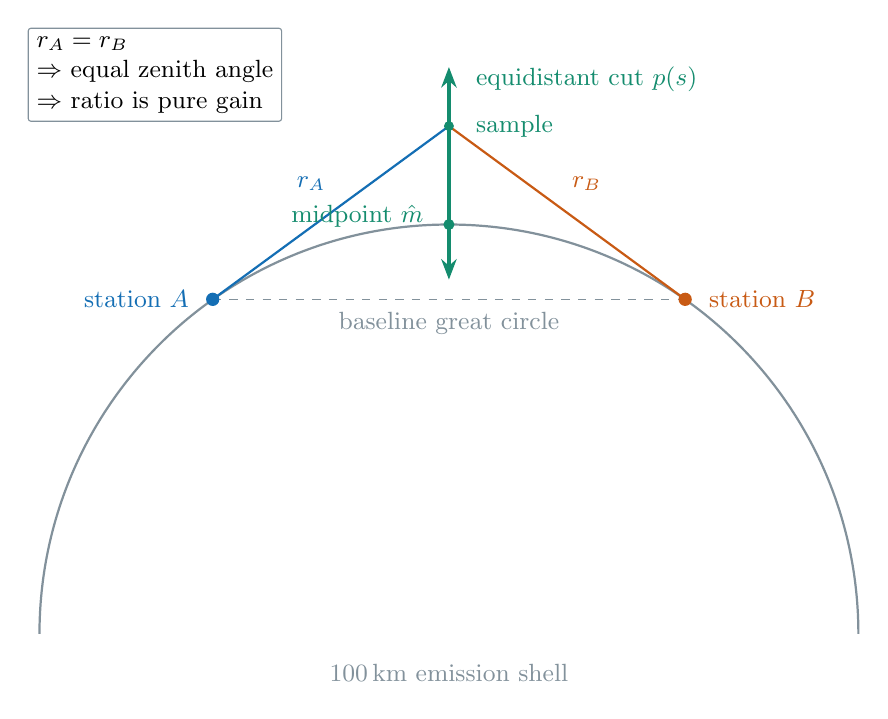
\begin{tikzpicture}[scale=1.0]
  \draw[soft,thick] (-5.2,0) arc (180:0:5.2);
  \node[soft,font=\small] at (0,-0.5) {\SI{100}{km} emission shell};
  \coordinate (A) at (-3.0,4.25);
  \coordinate (B) at (3.0,4.25);
  \coordinate (M) at (0,5.2);
  \coordinate (P) at (0,6.45);
  % station-station baseline
  \draw[dashed,soft] (A) -- (B);
  \node[soft,font=\small,below=1pt] at (0,4.25) {baseline great circle};
  % the equidistant cut leaves the baseline plane; drawn here in projection
  \draw[cut,very thick,{Stealth[length=2.6mm]}-{Stealth[length=2.6mm]}] (0,4.5) -- (0,7.2);
  \node[cut,font=\small,anchor=west] at (0.22,7.05) {equidistant cut $p(s)$};
  % equal ranges to one sample
  \draw[camA,thick] (A) -- (P);
  \draw[camB,thick] (B) -- (P);
  \node[camA,font=\small] at (-1.75,5.72) {$r_A$};
  \node[camB,font=\small] at (1.75,5.72) {$r_B$};
  \fill[cut] (P) circle (1.8pt);
  \node[cut,font=\small,anchor=west] at (0.22,6.45) {sample};
  \fill[cut] (M) circle (2.0pt);
  \node[cut,font=\small,anchor=east] at (-0.2,5.3) {midpoint $\hat m$};
  \fill[camA] (A) circle (2.4pt);
  \node[camA,font=\small,anchor=east] at (-3.18,4.25) {station $A$};
  \fill[camB] (B) circle (2.4pt);
  \node[camB,font=\small,anchor=west] at (3.18,4.25) {station $B$};
  \node[draw=soft,fill=white,rounded corners=1pt,align=left,font=\small,
        anchor=north west,inner sep=3pt] at (-5.35,7.7)
    {$r_A=r_B$\\ $\Rightarrow$ equal zenith angle\\ $\Rightarrow$ ratio is pure gain};
\end{tikzpicture}
\caption{The comparison locus. Every sample on the equidistant cut is the same
distance from both stations, so both cameras view it at the same zenith angle
and the measured ratio is free of view-angle response. The cut is the great
circle with pole $\hat a-\hat b$ through the midpoint.}
\label{fig:geometry}
\end{figure}

\subsection{Co-located instruments}

Sixteen of the seventy overlapping pairs are instruments sharing a station
(Gillam, Fort Smith, Pinawa, Rabbit Lake, Rankin Inlet, Yellowknife, Kiruna,
Oslo, Kristiansand). For these $\hat a=\hat b$, the equidistance condition holds
\emph{everywhere}, the pole $\hat n$ is undefined, and the cut direction is
unconstrained. GAIA takes it along the magnetic meridian plane, whose horizontal
trace at the station is magnetic north, i.e.\ azimuth equal to the local IGRF
declination.

These pairs are the best-conditioned measurements in the network: zero
parallax, identical viewing geometry, identical airmass, and no time-of-flight
mismatch between the two views of a moving structure. They should be weighted
accordingly, and they are the natural place to validate the whole pipeline
before trusting separated pairs.

\section{Paired keograms}

At each usable time step, sample~\eqref{eq:cut} at $N$ points in both cameras
and store the two profiles as rows. Stacking rows over time gives a pair of
keograms with identical spatial and temporal axes --- skewed relative to the
usual magnetic-meridian keogram because the cut is oriented by the station pair
(Fig.~\ref{fig:keogram}).

A practical note that makes this cheap: a projection mesh depends on the
calibration, station location and crop/mask, but \emph{never} on time. Each cut
point is therefore located in each camera's mesh once, yielding fixed texture
coordinates; every subsequent frame costs one texture read per sample rather
than a re-mesh. Extracting a 24-hour, 5-minute-cadence, $N=128$ keogram pair is
$\sim\!580$ small texture reads.

\begin{figure}[t]
\centering
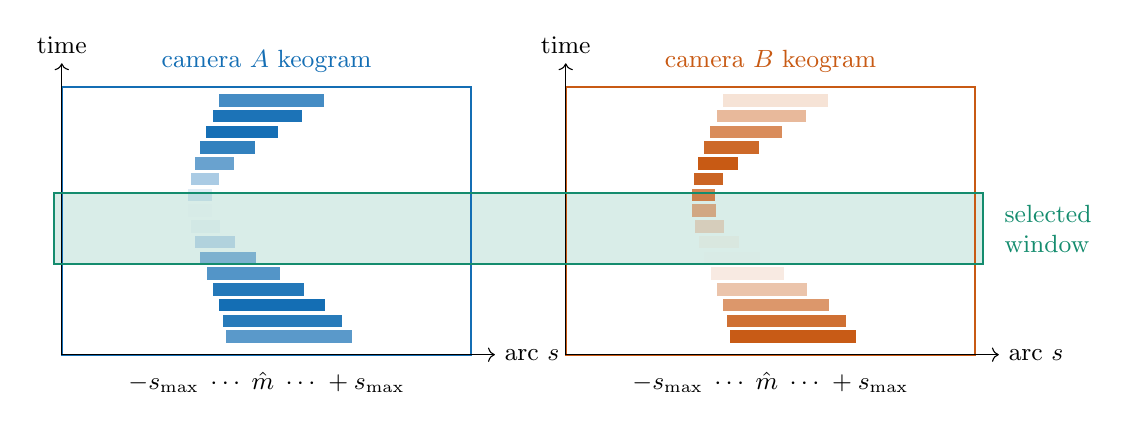
\begin{tikzpicture}[scale=1.0]
 \foreach \dx/\name/\col in {0/camera $A$/camA, 6.4/camera $B$/camB}{
  \begin{scope}[shift={(\dx,0)}]
   \draw[\col,thick] (0,0) rectangle (5.2,3.4);
   \node[\col] at (2.6,3.72) {\small \name{} keogram};
   % fake structure
   \foreach \y in {0.15,0.35,...,3.25}{
     \pgfmathsetmacro\a{0.5+0.5*sin(\y*160+\dx*12)}
     \pgfmathsetmacro\w{0.5+0.35*cos(\y*97)}
     \fill[\col,opacity=\a] (1.5+0.7*\w,\y) rectangle ++(1.9*\w,0.16);
   }
   \draw[->] (0,0) -- (5.5,0) node[right,font=\small] {arc $s$};
   \draw[->] (0,0) -- (0,3.7) node[above,font=\small] {time};
   \node[font=\small] at (2.6,-0.35) {$-s_{\max}\;\cdots\;\hat m\;\cdots\;+s_{\max}$};
  \end{scope}}
 % selection band across both
 \begin{scope}[on background layer]
  \fill[cut,opacity=0.16] (-0.1,1.15) rectangle (11.7,2.05);
 \end{scope}
 \draw[cut,thick] (-0.1,1.15) rectangle (11.7,2.05);
 \node[cut,right,font=\small,align=left] at (11.85,1.6)
   {selected\\ window};
\end{tikzpicture}
\caption{A pair of skew keograms: the same equidistant cut sampled by both
cameras, stacked over time. The user brushes a time window (green); only rows
inside it enter the fit. Both panels share spatial and temporal axes, so a row
pair is a set of simultaneous, co-located intensity measurements.}
\label{fig:keogram}
\end{figure}

\section{Estimating sensitivity and background}
\label{sec:estimation}

Within a selected window, every valid sample contributes a pair
$(J_B, J_A)$ of linearised intensities of the same sky point. From
\eqref{eq:model},
\begin{equation}
  J_A \;=\; \alpha_{AB} J_B + \beta_{AB},
  \qquad
  \alpha_{AB}=\frac{\gain_A}{\gain_B},
  \qquad
  \beta_{AB}=\off_A-\alpha_{AB}\off_B .
  \label{eq:pairfit}
\end{equation}
So one straight-line fit per pair yields both the relative sensitivity (slope)
and a combination of the backgrounds (intercept). The whole problem is a
straight-line fit --- but which fit matters a great deal.

\subsection{Ordinary least squares is the wrong estimator}

Both axes are noisy: this is an errors-in-variables problem, not a regression of
a noisy response on a clean predictor. Regressing $J_A$ on $J_B$ attenuates the
slope by the reliability ratio
\begin{equation}
  \mathbb{E}[\hat\alpha_{\text{OLS}}] \;\approx\;
  \alpha\,\frac{\sigma_S^2}{\sigma_S^2+\sigma_B^2},
\end{equation}
i.e.\ it is biased toward zero whenever the reference camera has appreciable
noise, and the bias grows precisely in the faint scenes we most want to
correct. Table~\ref{tab:estimators} shows the effect on a synthetic sample with
known truth ($\alpha=1.550$, $\beta=4.70$), 46 clean points and 3 injected
cloud/star outliers.

\begin{table}[h]
\centering
\begin{tabular}{lcc}
\toprule
Estimator & $\hat\alpha$ & error \\
\midrule
OLS, $J_A$ on $J_B$              & 1.190 & $-23\%$ \\
OLS, $J_B$ on $J_A$, inverted    & 1.728 & $+12\%$ \\
Reduced major axis (geometric mean) & 1.434 & $-7.5\%$ \\
Theil--Sen (robust, but still $y|x$) & 1.386 & $-11\%$ \\
\textbf{Deming, $\delta=\sigma_A^2/\sigma_B^2=1.21$} & \textbf{1.511} & $\mathbf{-2.5\%}$ \\
Deming after a naive $3\times$median-residual trim & 1.449 & $-6.5\%$ \\
\bottomrule
\end{tabular}
\caption{Slope recovery on synthetic data with truth $\alpha=1.550$. The two
one-sided OLS fits bracket the truth; orthogonal (Deming) regression with a
sensible noise ratio is much closer. Note the last row: trimming outliers using
residuals from a \emph{biased} preliminary fit made the answer worse than not
trimming at all.}
\label{tab:estimators}
\end{table}

\paragraph{Recommendation.} Use \textbf{Deming (orthogonal) regression} with the
variance ratio $\delta=\sigma_A^2/\sigma_B^2$ estimated from the cameras' own
read noise and exposure, defaulting to $\delta=1$ for identical models:
\begin{equation}
  \hat\alpha=\frac{(S_{yy}-\delta S_{xx})+\sqrt{(S_{yy}-\delta S_{xx})^2+4\delta S_{xy}^2}}{2S_{xy}},
  \qquad \hat\beta=\bar y-\hat\alpha\bar x .
\end{equation}
Apply robustness as \emph{iteratively reweighted} Deming on the orthogonal
residuals (Huber weights), never as a pre-trim keyed to a one-sided fit ---
Table~\ref{tab:estimators} shows why. Report the fitted $\hat\alpha$ with its
standard error; that error is what weights the network solve.

\begin{figure}[t]
\centering
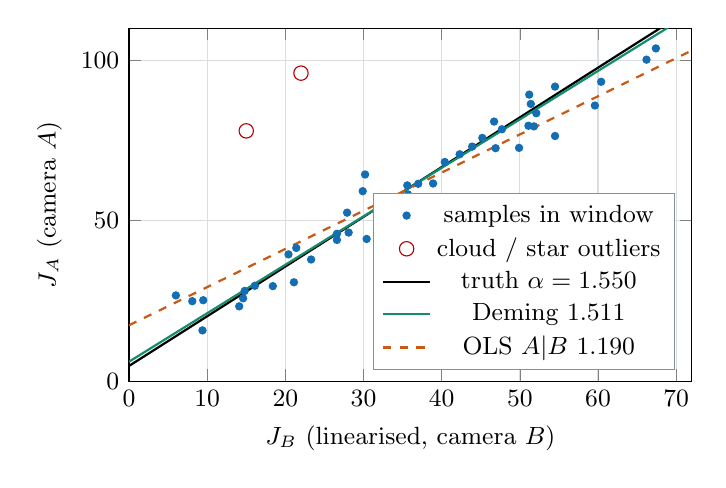
\begin{tikzpicture}
\begin{axis}[width=0.72\textwidth,height=0.5\textwidth,
  xlabel={$J_B$ (linearised, camera $B$)}, ylabel={$J_A$ (camera $A$)},
  xmin=0,xmax=72,ymin=0,ymax=110, grid=both, grid style={soft!30},
  legend pos=south east, legend style={font=\small,draw=soft,fill=white},
  tick label style={font=\small}, label style={font=\small}]
 \addplot[only marks,mark=*,mark size=1.3pt,camA] coordinates {
  (46.9,72.6) (52.1,83.5) (26.6,44.0) (30.4,44.3) (38.9,61.6) (67.4,103.7)
  (8.1,24.9) (30.2,64.4) (51.4,86.4) (35.7,58.2) (14.8,28.1) (20.4,39.5)
  (54.5,91.8) (16.1,29.7) (26.6,45.9) (34.2,48.8) (27.9,52.5) (36.0,56.0)
  (51.2,89.3) (6.0,26.7) (60.4,93.3) (49.9,72.7) (35.6,61.0) (21.1,30.8)
  (54.5,76.4) (37.0,61.5) (42.3,70.7) (28.1,46.3) (45.2,75.8) (66.2,100.2)
  (47.7,78.5) (14.1,23.3) (59.6,85.9) (14.6,25.8) (51.8,79.4) (40.4,68.3)
  (29.9,59.2) (39.7,53.9) (43.9,73.1) (9.4,15.8) (51.1,79.6) (9.5,25.2)
  (23.3,37.9) (21.4,41.5) (18.4,29.6) (46.7,80.9)};
 \addlegendentry{samples in window}
 \addplot[only marks,mark=o,mark size=2.6pt,red!70!black] coordinates {(22.0,96.0) (58.0,41.0) (15.0,78.0)};
 \addlegendentry{cloud / star outliers}
 \addplot[thick,black,domain=0:72] {1.550*x+4.70};
 \addlegendentry{truth $\alpha=1.550$}
 \addplot[thick,cut,domain=0:72] {1.511*x+6.03};
 \addlegendentry{Deming $1.511$}
 \addplot[thick,dashed,camB,domain=0:72] {1.190*x+17.39};
 \addlegendentry{OLS $A|B$ $1.190$}
\end{axis}
\end{tikzpicture}
\caption{Why the estimator matters. The slope is the relative sensitivity
$\gain_A/\gain_B$ and the intercept encodes the background difference. Ordinary
least squares (dashed) is pulled systematically flat because the abscissa is
noisy; orthogonal regression tracks the truth closely.}
\label{fig:scatter}
\end{figure}

\subsection{Background structure}

$\off_c$ is not a constant. Light pollution rises toward a populated horizon,
twilight leaves a gradient across the field, and scattered moonlight moves. Two
mitigations, in order of value:
\begin{enumerate}
  \item \textbf{Gate on darkness.} Require solar elevation below $-12^\circ$ at
    \emph{both} stations. GAIA already computes exactly this quantity for the
    twilight weight, so the gate is free.
  \item \textbf{Allow a first-order spatial term.} Extend~\eqref{eq:pairfit} to
    $J_A=\alpha J_B+\beta_0+\beta_1 s$, with $s$ the arc length along the cut.
    One extra parameter absorbs a linear background gradient (city glow at one
    end, twilight at the other) that would otherwise leak into $\alpha$. Fit it
    by default and report $\beta_1$; a large $\beta_1$ is a warning that the
    window is contaminated.
\end{enumerate}
Do \emph{not} attempt to fit a per-camera response curve $f_c$ from auroral
scenes. Three-parameter (gain, offset, gamma) fits on this data are badly
conditioned and will trade gamma against gain.

\subsection{Colour channels}

Offer both modes, as requested, and default to per-channel:
\begin{itemize}
  \item \textbf{Per channel.} Fit $(\alpha,\beta)$ independently for $R$, $G$,
    $B$. This is the physically correct choice: the cameras differ in filter
    passband and colour balance, not merely in overall level, and the aurora is
    strongly chromatic (\SI{557.7}{nm} versus \SI{630.0}{nm} versus the blue
    $\mathrm{N_2^+}$ bands). Per-channel gains also correct hue steps across
    overlaps, which the eye notices more readily than brightness steps.
  \item \textbf{Single average.} Fit one $(\alpha,\beta)$ on the channel mean.
    More robust when a channel is nearly dark or saturated, and the right choice
    for monochrome instruments and for narrowband cameras where a colour ratio
    is meaningless.
\end{itemize}
Guard the per-channel mode: if a channel's dynamic range in the window is below
a threshold, fall back to the average for that channel rather than returning a
wild gain.

\section{Selecting subsets of paired cameras}
\label{sec:selection}

Of $43$ calibrated, located cameras, $70$ pairs have overlapping coverage
(station separation below $2\times\SI{373}{km}$, twice the ground reach at the
$75^\circ$ taper knee). The separation distribution is strongly bimodal
(Fig.~\ref{fig:hist}): co-located clusters, then a gap, then genuinely separated
pairs.

\begin{figure}[h]
\centering
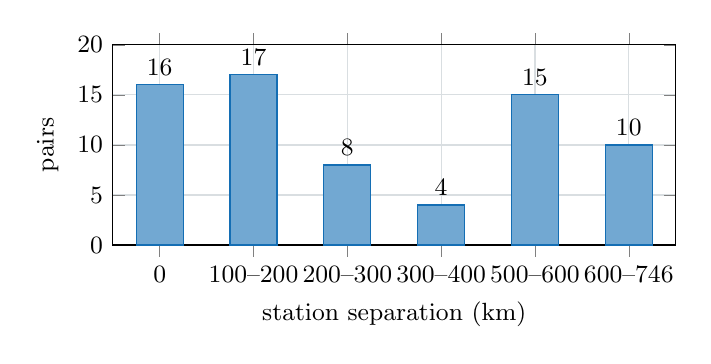
\begin{tikzpicture}
\begin{axis}[width=0.72\textwidth,height=0.34\textwidth,
  ybar,bar width=17pt, xlabel={station separation (km)}, ylabel={pairs},
  ymin=0, ymax=20, xtick=data, symbolic x coords={0,100--200,200--300,300--400,500--600,600--746},
  nodes near coords, every node near coord/.append style={font=\small},
  tick label style={font=\small}, label style={font=\small},
  grid=both, grid style={soft!30}]
 \addplot[fill=camA!60,draw=camA] coordinates
   {(0,16) (100--200,17) (200--300,8) (300--400,4) (500--600,15) (600--746,10)};
\end{axis}
\end{tikzpicture}
\caption{Separation of the 70 overlapping pairs. The 16 pairs at \SI{0}{km} are
co-located instruments and are the best-conditioned comparisons available.}
\label{fig:hist}
\end{figure}

Selection should happen at two levels.

\paragraph{Automatic gating (per pair, per window).} Admit a window only if all
of Table~\ref{tab:gates} hold. The network is heavily redundant
(Sec.~\ref{sec:network}), so it is far better to be strict and discard than to
admit marginal data.

\begin{table}[h]
\centering
\small
\begin{tabular}{p{0.30\textwidth}p{0.28\textwidth}p{0.34\textwidth}}
\toprule
Criterion & Suggested threshold & Why \\
\midrule
Darkness at both stations & solar elevation $<-12^\circ$ & background otherwise
dominated by twilight gradient; quantity already computed \\
Frame simultaneity & $|t_A-t_B|<\SI{30}{s}$ & auroral forms move at
$\sim\!\SI{1}{km/s}$; \SI{30}{s} is \SI{30}{km} of smear at the shell \\
Cut coverage & $\geq 60\%$ of samples valid in both meshes & short cuts give
little leverage and are dominated by mesh edges \\
Dynamic range & robust IQR of $J_B$ above a floor & a uniformly dark window
cannot constrain a slope at all; \emph{structure is required} \\
Cloud & \texttt{quality.rs} cloud probability below threshold at both & cloud
decorrelates the two views and breaks the shared-$S$ assumption \\
Moon & below horizon, or large angular distance from the cut & scattered
moonlight is a strong, moving background \\
Saturation & fraction of samples at 0 or 255 below a few percent & clipped
samples bias both slope and intercept \\
\bottomrule
\end{tabular}
\caption{Automatic admission gates for a candidate pair-window.}
\label{tab:gates}
\end{table}

\paragraph{Manual subsetting (the interface).} The operator needs to work with
sets, not one pair at a time. Provide:
\begin{itemize}
  \item the pair list filtered by \emph{station} (all pairs involving camera
    $X$) --- the natural entry point from the Cameras tab;
  \item filters for \emph{co-located only} and \emph{separated only}, since the
    two behave very differently and co-located pairs are the validation set;
  \item selection by \emph{connected group}, because a solve is only meaningful
    within a group and each group needs its own anchor;
  \item a quality column (samples, $\hat\alpha$ standard error, $\beta_1$,
    cloud flag) so the operator can sort and exclude by evidence rather than by
    intuition;
  \item and a shared time window applied across all selected pairs, so one
    quiet, structured, moonless interval drives the whole solve.
\end{itemize}

\section{From pair ratios to camera constants}
\label{sec:network}

Pairwise ratios are mutually inconsistent in general: measured $\alpha_{AC}$
will not equal $\alpha_{AB}\alpha_{BC}$. Resolve this by a least-squares solve
over each connected group. Both unknowns reduce to the \emph{same} structure.

\paragraph{Gains.} Taking logarithms of $\alpha_{ij}=\gain_i/\gain_j$ makes the
constraints linear:
\begin{equation}
  \min_{\ln \gain}\;\sum_{(i,j)\in E} w_{ij}\bigl(\ln \gain_i-\ln \gain_j-\ln\hat\alpha_{ij}\bigr)^2,
  \qquad \text{subject to}\quad \sum_{i\in G}\ln \gain_i=0 .
  \label{eq:gainsolve}
\end{equation}
The design matrix is the graph incidence matrix, so the normal equations are a
weighted graph Laplacian system $L\,\ln \gain = d$, positive semi-definite with a
one-dimensional null space --- exactly the gauge freedom, removed by the
constraint.

\paragraph{Offsets.} Substituting $\alpha_{ij}=\gain_i/\gain_j$ into
$\beta_{ij}=\off_i-\alpha_{ij}\off_j$ and dividing by $\gain_i$:
\begin{equation}
  \frac{\beta_{ij}}{\gain_i}
  \;=\; \frac{\off_i}{\gain_i}-\frac{\off_j}{\gain_j}
  \;=\; c_i-c_j,
  \qquad c_c\equiv\frac{\off_c}{\gain_c}.
\end{equation}
So in the reduced variable $c=\off/\gain$ the offsets satisfy the identical
incidence structure and are obtained from a second Laplacian solve with the same
matrix and a different right-hand side. \textbf{One solver does both.}

\paragraph{Redundancy and consistency.} The graph is far from a tree, which is
good news. Group~1 has $V=11$, $E=27$ ($17$ independent cycles); group~2 has
$V=8$, $E=28$ ($21$ cycles). Every independent cycle is a closure test: the sum
of $\ln\hat\alpha$ around it should vanish, and its residual is a direct,
assumption-free measure of inconsistency. Surface the per-cycle residuals in the
interface; they detect a bad pair far more reliably than any single fit
diagnostic.

\paragraph{Gauge and unreachable cameras.} Fifteen groups exist, of sizes
$11,8,4,3,3,3,2,2$ and seven singletons. Choose the gauge deliberately: either
anchor on the best-characterised instrument in each group, or set the weighted
median $\ln \gain$ to zero so no single camera's error propagates to all others.
The seven isolated cameras have no overlapping partner and therefore
\emph{cannot} be equalized by this method at all; they must keep $\gain=1,
\off=0$ and be labelled as such in the interface. Groups are also independent:
there is no way to tie the Fennoscandian and North American clusters together
photometrically without a common view.

\begin{figure}[t]
\centering
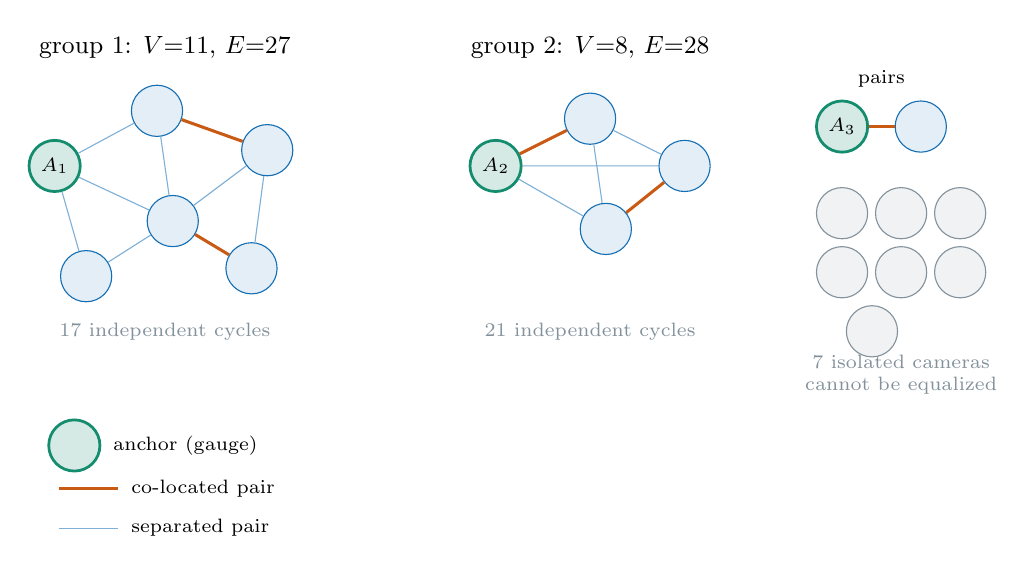
\begin{tikzpicture}[
  cam/.style={circle,draw=camA,fill=camA!12,minimum size=6.5mm,inner sep=0,font=\scriptsize},
  anch/.style={circle,draw=cut,line width=1pt,fill=cut!18,minimum size=6.5mm,inner sep=0,font=\scriptsize},
  iso/.style={circle,draw=soft,fill=soft!12,minimum size=6.5mm,inner sep=0,font=\scriptsize},
  e/.style={draw=camA!55}, co/.style={draw=camB,line width=1.1pt}]
 % group 1
 \node[anch] (a1) at (0,1.5) {$A_1$};
 \node[cam] (a2) at (1.3,2.2) {};  \node[cam] (a3) at (1.5,0.8) {};
 \node[cam] (a4) at (2.7,1.7) {};  \node[cam] (a5) at (2.5,0.2) {};
 \node[cam] (a6) at (0.4,0.1) {};
 \draw[e] (a1)--(a2) (a1)--(a3) (a2)--(a4) (a3)--(a4) (a3)--(a5) (a4)--(a5) (a1)--(a6) (a3)--(a6) (a2)--(a3);
 \draw[co] (a2)--(a4); \draw[co] (a3)--(a5);
 \node[font=\small] at (1.4,3.0) {group 1: $V{=}11$, $E{=}27$};
 \node[font=\scriptsize,soft] at (1.4,-0.6) {17 independent cycles};
 % group 2
 \begin{scope}[shift={(5.6,0)}]
  \node[anch] (b1) at (0,1.5) {$A_2$};
  \node[cam] (b2) at (1.2,2.1) {}; \node[cam] (b3) at (1.4,0.7) {};
  \node[cam] (b4) at (2.4,1.5) {};
  \draw[e] (b1)--(b2) (b1)--(b3) (b2)--(b3) (b2)--(b4) (b3)--(b4) (b1)--(b4);
  \draw[co] (b1)--(b2); \draw[co] (b3)--(b4);
  \node[font=\small] at (1.2,3.0) {group 2: $V{=}8$, $E{=}28$};
  \node[font=\scriptsize,soft] at (1.2,-0.6) {21 independent cycles};
 \end{scope}
 % small groups + singletons
 \begin{scope}[shift={(10.0,0)}]
  \node[anch] (c1) at (0,2.0) {$A_3$}; \node[cam] (c2) at (1.0,2.0) {};
  \draw[co] (c1)--(c2);
  \node[font=\scriptsize] at (0.5,2.6) {pairs};
  \node[iso] at (0,0.9) {}; \node[iso] at (0.75,0.9) {}; \node[iso] at (1.5,0.9) {};
  \node[iso] at (0,0.15) {}; \node[iso] at (0.75,0.15) {}; \node[iso] at (1.5,0.15) {};
  \node[iso] at (0.38,-0.6) {};
  \node[font=\scriptsize,soft,align=center] at (0.75,-1.15) {7 isolated cameras\\ cannot be equalized};
 \end{scope}
 \node[anch] at (0.25,-2.05) {};
 \node[right,font=\scriptsize] at (0.62,-2.05) {anchor (gauge)};
 \draw[co] (0.05,-2.6) -- ++(0.75,0);
 \node[right,font=\scriptsize] at (0.85,-2.6) {co-located pair};
 \draw[e] (0.05,-3.1) -- ++(0.75,0);
 \node[right,font=\scriptsize] at (0.85,-3.1) {separated pair};
\end{tikzpicture}
\caption{Schematic of the overlap graph. Gains and offsets are determined only
within a connected group and only up to one anchor per group. Cycles provide
closure tests; co-located edges (orange) are the most reliable constraints.
Node counts are the real ones; layout is schematic.}
\label{fig:graph}
\end{figure}

\section{Applying the result in the composite}

With $(\gain_c,\off_c)$ known, correct each camera to the common scale
\emph{before} averaging, and do it in linear space:
\begin{equation}
  \boxed{\;
  \text{out}(p) \;=\; f\!\left(
    \frac{\sum_c w_c(p)\,\dfrac{f_c^{-1}\bigl(I_c(p)\bigr)-\off_c}{\gain_c}}
         {\sum_c w_c(p)}\right)\;}
  \label{eq:apply}
\end{equation}
Three points of implementation discipline:
\begin{itemize}
  \item The gain is \textbf{not} a fifth weight. The existing four factors
    multiply $w_c$ and cancel for a single contributor; $\gain_c$ and $\off_c$
    multiply and shift the \emph{value} and must not enter the denominator.
  \item Equation~\eqref{eq:apply} requires the linearisation
    $f_c^{-1}$ discussed in Sec.~1. This is a change to the current
    encoded-space average and should be made in the same commit, since applying
    gains in encoded space would introduce its own error.
  \item Clamp and record. Store $(\gain,\off)$ per camera per channel with the
    window and method that produced them, and publish them in the manifest's
    \texttt{stitching} block, as the four weight factors already are. A mosaic
    whose photometry has been adjusted must say so.
\end{itemize}

\section{Staged plan}

The geometry and sampling layer is already implemented and tested
(\texttt{backend/equalize.rs}): the equidistant cut, the co-located magnetic
meridian fallback, and once-per-camera mesh location giving fixed texture
coordinates. The remaining work splits into five stages, each independently
useful and independently checkable (Fig.~\ref{fig:pipeline}).

\begin{figure}[h]
\centering
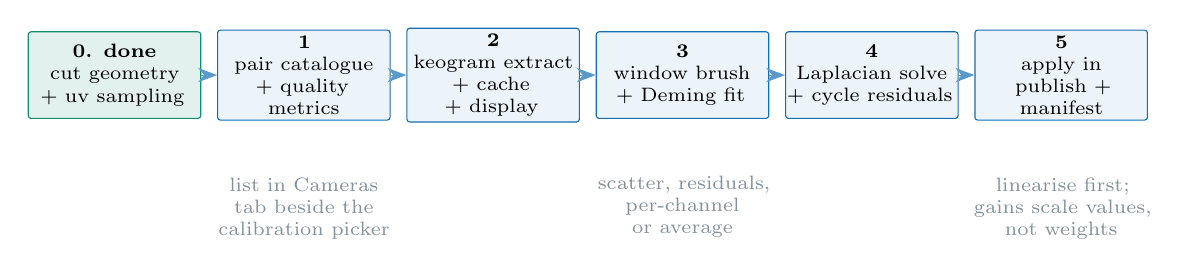
\begin{tikzpicture}[node distance=2mm,
  box/.style={draw=camA,fill=camA!8,rounded corners=1pt,align=center,font=\scriptsize,
              minimum height=11mm,text width=20.5mm,inner sep=2pt},
  done/.style={box,draw=cut,fill=cut!12},
  a/.style={-{Stealth[length=2.4mm]},camA!70}]
 \node[done] (s0) {\textbf{0. done}\\ cut geometry\\ + uv sampling};
 \node[box,right=of s0] (s1) {\textbf{1}\\ pair catalogue\\ + quality metrics};
 \node[box,right=of s1] (s2) {\textbf{2}\\ keogram extract\\ + cache + display};
 \node[box,right=of s2] (s3) {\textbf{3}\\ window brush\\ + Deming fit};
 \node[box,right=of s3] (s4) {\textbf{4}\\ Laplacian solve\\ + cycle residuals};
 \node[box,right=of s4] (s5) {\textbf{5}\\ apply in\\ publish + manifest};
 \draw[a] (s0)--(s1); \draw[a] (s1)--(s2); \draw[a] (s2)--(s3);
 \draw[a] (s3)--(s4); \draw[a] (s4)--(s5);
 \node[below=6mm of s1,font=\scriptsize,text width=24mm,align=center,soft] {list in Cameras tab beside the calibration picker};
 \node[below=6mm of s3,font=\scriptsize,text width=24mm,align=center,soft] {scatter, residuals, per-channel or average};
 \node[below=6mm of s5,font=\scriptsize,text width=24mm,align=center,soft] {linearise first; gains scale values, not weights};
\end{tikzpicture}
\caption{Staged implementation. Stage 0 exists; each later stage leaves the
system in a usable state and can be validated on co-located pairs before
separated ones are trusted.}
\label{fig:pipeline}
\end{figure}

\begin{enumerate}\setcounter{enumi}{0}
  \item[\textbf{Stage 1.}] Pair catalogue endpoint: enumerate overlapping pairs
    with separation, group id, and the gates of Table~\ref{tab:gates} evaluated
    for a default window. UI: a list in the Cameras tab beside the calibration
    picker, filtered to the selected camera. \emph{Check:} the counts reproduce
    $70$ pairs, $16$ co-located, $15$ groups.
  \item[\textbf{Stage 2.}] Keogram extraction and cache, keyed by pair, cut
    parameters, cadence and date. UI: the two keograms with shared axes.
    \emph{Check:} a co-located pair shows visually near-identical structure,
    which is the strongest available end-to-end validation of the geometry.
  \item[\textbf{Stage 3.}] Window selection and the pairwise fit: Deming with
    Huber reweighting, optional $\beta_1 s$ term, per-channel or average. UI:
    brush on the keogram, scatter plot with fit and residuals, reported standard
    errors. \emph{Check:} a co-located pair of identical instruments must return
    $\hat\alpha\approx1$, $\hat\beta\approx0$.
  \item[\textbf{Stage 4.}] Network solve per group with explicit gauge, plus
    per-cycle closure residuals. UI: a review table of $(\gain,\off)$ per camera
    per channel, isolated cameras clearly marked as not equalizable.
    \emph{Check:} closure residuals small; removing one pair should not move the
    solution much in the highly redundant groups.
  \item[\textbf{Stage 5.}] Apply via~\eqref{eq:apply} in \texttt{publish.rs},
    together with the move to linear-space averaging, and record the constants in
    the manifest. \emph{Check:} overlap seams measurably reduced --- quantify by
    the median absolute difference between contributing cameras along the
    equidistant cuts before and after.
\end{enumerate}

\section{Risks and open questions}

\begin{itemize}
  \item \textbf{Unknown response curves.} Assuming sRGB is a big improvement on
    assuming linearity, but it is still an assumption. Co-located pairs of
    \emph{different} instrument types are the only place to test it: a curved
    locus in Fig.~\ref{fig:scatter} rather than a straight line is the signature
    of mismatched $f_c$, and it should be surfaced rather than fitted away.
  \item \textbf{Time variability.} $\gain$ drifts with focus, icing and
    windowing changes; $\off$ varies nightly with moon and cloud. Constants
    should carry a validity interval exactly as calibrations do, not be treated
    as permanent.
  \item \textbf{Parallax for separated pairs.} Equidistance removes the
    view-angle term but not the fact that aurora is not a thin sheet at exactly
    \SI{100}{km}. Emission above or below the assumed shell projects to
    different ground points for the two cameras, and the mismatch grows with
    separation. Expect co-located pairs to be clean and long-baseline pairs to
    show irreducible scatter; weight accordingly and consider capping usable
    separation well below \SI{746}{km}.
  \item \textbf{Isolated cameras.} Seven cameras cannot be equalized at all.
    Either accept the step at their edges, or acquire an overlapping partner.
  \item \textbf{Do not couple this to the weights.} It is tempting to fold
    photometric correction into the weighting; that would silently change the
    meaning of the four existing factors and make both harder to reason about.
\end{itemize}

\end{document}
